\chapter{Usando teor\'ia de modelos}
\label{sec:intro_logica}

En el Cap\'itulo \ref{sec:intro} (Secci\'on \ref{sec:gre-teoria-modelos}) introdujimos terminiolog\'ia y conceptos b\'asicos de l\'ogica y de teor\'ia de modelos y motivamos su uso para GER.
De acuerdo a la complejidad de las estructuras gramaticales que querramos permitir en las ERs, tendremos un lenguaje asociado, 
el cual pertenecer\'a a alguna l\'ogica. En este cap\'itulo se explica c\'omo partiendo de f\'ormulas de primer orden (\FOL) 
podemos ir restringiendo la l\'ogica y con ello el lenguaje, y as\'i conseguir una menor complejidad computacional. Es interesante evaluar la complejidad dependiendo de la l\'ogica seleccionada, 
ya que, por ejemplo, sistemas de tiempo real necesitan conseguir ERs r\'apidamente. Daremos la complejidad de las distintas l\'ogicas, 
y veremos qu\'e l\'ogica aplica a cada algoritmo del estado del arte del \'area introducidos en el Cap\'itulo \ref{sec:seleccion}.

Este cap\'itulo esta dividido en 5 secciones. En la Secci\'on \ref{sec:seleccionandoLenguaje} daremos nociones de similaridad entre objetos del modelo en un lenguaje particular y explicamos como se relacionan con la GER. Pero como la similaridad involucra la verificaci\'on de infinitas f\'ormulas, veremos simulaciones que es un concepto matem\'atico que nos va a ayudar a resolver el problema de GER sin tener que verificar infinitas f\'ormulas. Luego en la Secci\'on \ref{sec:greViaSimulacion} veremos c\'omo computar ERs en \EL usando simulaciones. En la Secci\'on \ref{sec:bisimulacion} veremos c\'omo computar ERs en \ALC, y en la Secci\'on \ref{sec:computandoEnFOL} en \FOL. Para finalizar en la Secci\'on \ref{sec:notasFinales} daremos un res\'umen del cap\'itulo y contaremos como se linkea esta parte de la tesis con los dem\'as cap\'itulos.


\section{Objetos indistinguibles en un lenguaje l\'ogico $\+L$}
\label{sec:seleccionandoLenguaje}

En esta secci\'on veremos dos conceptos importantes, similaridad en $\+L$, y simulaci\'on en $\+L$. Recordemos que en la Secci\'on \ref{sec:gre-teoria-modelos} definimos el output del problema GER con el lenguaje $\+L$ (i.e. $\+L$-GER) como una f\'ormula $\phi$ en $\+L$ cuya interpretaci\'on en el modelo de entrada  $\+M$ es el conjunto target T, si esa f\'ormula existe. Formalmente, $\+L$-GER($\+M$, T)=\{$\phi$ en $\+L$ | $\interp{\phi}$ = T \} $\lor \perp$ en caso de no existir ninguna f\'ormula.

\subsection{Los objetos indistinguibles en $\+L$ son \emph{$\+L$-similares}}
\label{sec:indistinguibles}

Considere la Figura \ref{target_mapa_3ball}, asumamos que el lenguaje en el que podemos generar ERs, es decir, nuestro $\+L$, es $\CL$. $\CL$ es el lenguaje l\'ogico
que s\'olo puede tener conjunciones de propiedades proposicionales, 
sin negaci\'on, sin relaciones. Sea REL = $\{\nLarge, \nSmall, \nRed, \nBall, \nCube, \nYellow \}$ nuestro vocabulario, es decir, el conjunto de relaciones (unarias) que podemos usar en las ERs.
%\begin{figure}[h]
%\begin{subfigure}{.5\textwidth}
%\centering
%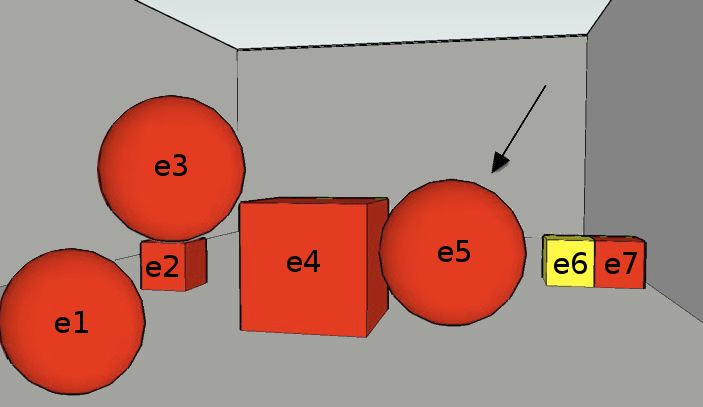
\includegraphics[width=.6\textwidth]{images/22paraRelacionalLetras.png}
%\caption{Ejemplo de contexto.}
%\label{target_mapa_3ball}
%\end{subfigure}

\begin{figure}[!ht]
\begin{subfigure}{.5\textwidth}

\centering
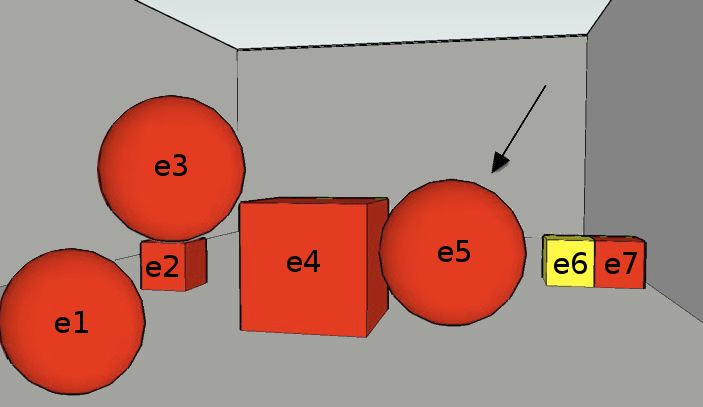
\includegraphics[width=\textwidth]{images/22paraRelacionalLetras.png}\\[0pt]
%\caption{Ejemplo de contexto.}
\end{subfigure}
\hspace*{0cm}
\begin{subfigure}{.5\textwidth}

%\begin{subfigure}{.5\textwidth}
  \centering
\vspace*{1cm}
\begin{picture}(250,50)
\put(0,-50){\begin{tikzpicture}
  [
    n/.style={circle,draw,inner sep=1.5pt,node distance=1.5cm},
		 aArrow/.style={->, >=stealth, semithick, shorten <= 1pt, shorten >= 1pt},
  ]
 \node[n,label=below:{
    \relsize{-2}$\begin{array}{c}
      \nLarge\\[-3pt] 
      \nRed \\[-3pt] 
      \nBall\end{array}$}] (a) {$e_1$};
 \node[n,label=below:{
    \relsize{-2}$\begin{array}{c}     
      \nSmall\\[-3pt] 
      \nRed\\[-3pt] 
      \nCube\end{array}$}, right of=a] (b) {$e_2$};
 \node[n,label=above:{
    \relsize{-2}$\begin{array}{c}     
      \nLarge\\[-3pt] 
      \nRed\\[-3pt] 
      \nBall\end{array}$}, above of=b] (c) {$e_3$};
 \node[n,label=below:{
    \relsize{-2}$\begin{array}{c}
      \nLarge\\[-3pt] 
      \nRed\\[-3pt] 
      \nCube\end{array}$}, right of=b] (d) {$e_4$};
 \node[n,label=below:{
    \relsize{-2}$\begin{array}{c}
      \nLarge\\[-3pt] 
      \nRed\\[-3pt] 
      \nBall\end{array}$}, right of=d] (e) {$e_5$};
 \node[n,label=below:{
    \relsize{-2}$\begin{array}{c}
      \nSmall\\[-3pt] 
      \nYellow\\[-3pt] 
      \nCube\end{array}$}, right of=e] (f) {$e_6$};
 \node[n,label=below:{
    \relsize{-2}$\begin{array}{c}
      \nSmall\\[-3pt]
      \nRed\\[-3pt] 
      \nCube\end{array}$},  right of=f] (g) {$e_7$};
 %\draw [aArrow,bend right=40] (b) to node[auto,swap]{\relsize{-3}$\nBelow$} (c);
 %\draw [aArrow,bend right=40] (c) to node[auto,swap]{\relsize{-3}$\nOntop$} (b);
 %\draw [aArrow,bend right=40] (d) to node[auto,swap]{\relsize{-3}$\nLeftof$} (e);
 %\draw [aArrow,bend right=40] (e) to node[auto,swap]{\relsize{-3}$\nRightof$} (d);
 %\draw [aArrow,bend right=40] (f) to node[auto,swap]{\relsize{-3}$\nLeftof$} (g);
 %\draw [aArrow,bend right=40] (g) to node[auto,swap]{\relsize{-3}$\nRightof$} (f);
 %\draw[dotted] (-0.5,-1.3) rectangle (8,3.1);
 \draw[dotted] (-0.5,-1.5) rectangle (8,3);
 \end{tikzpicture}}
 \end{picture}
 %\end{flushleft}

\vspace*{2cm} 
% \caption{}\label{representacion-modelo}

%\end{subfigure}%

\label{representacion-modelo}
\end{subfigure}
\caption{Contexto y modelo s\'olo con propiedades proposicionales.}\label{target_mapa_3ball}

\end{figure}
Ahora si buscamos una ER para el target T = \{$e_5$\} en la Figura \ref{target_mapa_3ball} usando el lenguaje $\+C$, veremos que no existe una ER en $\+C$ para $e_5$. Observando el modelo de la figura vemos que todas las f\'ormulas que son ciertas de $e_5$ y sus interpretaciones son las siguientes:

\begin{itemize}
\item Con 1 proposici\'on: $\interp{\nRed}$=\{$e_1$,$e_2$,$e_3$,$e_4$,$e_5$,$e_7$\}, $\interp{\nLarge}$=\{$e_1$,$e_3$,$e_4$,$e_5$\}, $\interp{\nBall}$=\{$e_1$,$e_3$,$e_5$\},\\
$\interp{\nYellow}$=\{$e_6$\}
\item Con 2 proposiciones: $\interp{\nRed \land \nBall}$=\{$e_1$,$e_3$,$e_5$\}, $\interp{\nBall \land \nLarge}$=\{$e_1$,$e_3$,$e_5$\}, $\interp{\nYellow \land \nCube}$=\{$e_6$\}  \\
      $\interp{\nLarge \land \nRed}$=\{$e_1$,$e_3$,$e_4$,$e_5$\}
\item Con 3 proposiciones: $\interp{\nLarge \land \nRed \land \nBall}$=\{$e_1$,$e_3$,$e_5$\}
\end{itemize}

Conclu\'imos que $e_5$ no puede distinguirse de $e_1$ y $e_3$ usando s\'olo propiedades proposicionales y conjunci\'on que es lo que $\+C$ nos permite. Decimos que $e_5$ es $\+C$-similar a $e_1$ y a $e_3$ y por lo tanto no es posible identificar un\'ivocamente a $e_5$ usando el lenguaje $\+C$.
%\floatname{definition}{Definici\'on}
\newtheorem{definicion}{Definici\'on}
\begin{definicion}

En general, dado un lenguaje l\'ogico $\+L$ decimos que un objeto $u$ en un modelo
$\+M$ es {\bf $\+L$-similar} a otro objeto
 $v$ del modelo si para toda f\'ormula en $\+L$ satisfecha por $u$ tambi\'en es satisfecha por $v$. 
\end{definicion}

%Siguiendo la notaci\'on de~\cite{areces08} usamos \emph{$u$ es $\+L$-similar a $v$} para decir que $u$ es $\+L$-similar a $v$.

Formalmente sea $\+M = \tup{\Delta, \interp{\cdot}}$ un modelo relacional con $u$, $v \in \Delta$
$u \simil{\+L} v$ ($u~\+L$-similar $v$) si para toda f\'ormula $\phi$ en $\+L$, $u \in \interp{\phi} \Rightarrow v \in \interp{\phi}$. 
La $\+L$-similaridad captura la noci\'on de ``capacidad de identificar en $\+L$''. 

%Se cumple que  $e_1 \simil{\+L} e_5$, $e_3 \simil{\+L} e_5$ y $e_1 \simil{\+L} e_3$ ya que para toda f\'omula $\phi$, la {\bf interpretaci\'on de la f\'ormula} ($\interp \phi$) es $\{e_1, e_3, e_5\}$. 
%$\phi_1$: $\nRed \land \nBall$ tenemos que $\interp {\phi_1} $= $\{e_1, e_3, e_5\}$
%
%$\phi_2$: $\nLarge \land \nBall$, $\interp {\phi_2} $ = $\{e_1, e_3, e_5\}$
%
%$\phi_3$: $\nRed \land \nLarge \land \nBall$, $\interp {\phi_3}$ = $\{e_1, e_3, e_5\}$
%
%Esto nos dice que con ese lenguaje elegido $\+L$ la tarea GER con target $e_5$ no tiene soluci\'on.

La noci\'on de $\+L$-similaridad entonces, nos permite identificar aquellos elementos del modelo que pueden o no ser referenciados usando un lenguaje dado $\+L$. En 
la Figura \ref{target_mapa_3ball} s\'olo $e_4$ ({\it el cubo grande}) y $e_6$ ({\it el cubo amarillo}) pueden ser referenciados en $\+C$. Y por lo tanto, nos permitir\'ia identificar qu\'e lenguaje es necesario para poder generar ERs para los elementos de un modelo dado. En nuestro ejemplo tenemos que $e_5 \simil{\+C} e_1$ y $e_5 \simil{\+C} e_3$. Por lo que $\+C$-GER no tiene soluci\'on, para este ejemplo es $\perp$. Si usamos un lenguaje m\'as expresivo como $\EL$ que permite usar relaciones binarias, la f\'ormula $\nBall \land \exists\nRightof. \nCube$ es una ER para el target del ejemplo. 

Sin embargo, no es posible computar $\EL$-GER para nuestro ejemplo dado que, como est\'a planteada, la noci\'on de $\+L$-similaridad requer\'ia computar infinitas f\'ormulas. Las f\'ormulas en $\EL$ que describen al target $e_5$ son infinitas porque hay un ciclo en el modelo.

La soluci\'on para no tener que considerar infinitas f\'ormulas es reformular la noci\'on de $\+L$-similaridad de una manera estructural usando la noci\'on de teor\'ia de modelos conocida como {\bf $\+L$-simulaci\'on}. A diferencia de la $\+L$-similaridad que se define sobre infinitas f\'ormulas, las $\+L$-simulaciones se definen sobre el modelo, el cual para la GER, es finito.

\subsection{Los objetos indistinguibles son \emph{$\+L$-simulables}}

La relaci\'on entre $\+L$-similaridad y $\+L$-simulaci\'on ha sido ampliamente estudiada y el siguiente es un resultado fundamental de teor\'ia de modelos:


\newtheorem{teorema}{Teorema}
%$Una l\'ogica sim\'etrica cumple  $\atomL$ y $\atomR$ como se ve en la Tabla \ref{tab:simuls}. 
\begin{teorema} \label{thm:simulation}
Si  $\+M = \tup{\Delta, \interp{\cdot}}$ es un modelo finito, $u$ y $v \in \Delta$, entonces $u \simil{\+L} v$ ($u~\+L$-similar $v$) si y s\'olo si 
$u \simul{\+L} v$ ($u~\+L$-simula $v$) (para $\+L \in \cset{\FOL,\EPFOL,\ALC,\EL,\ELAN}$).
\end{teorema}

Demostraci\'on tomada de \cite{arec:usin11} p\'agina 34: $\simul{\FOL}$ es isomorfismo en
grafos etiquetados~\cite{ebbi:math96}; $\simul{\ALC}$ corresponde a la
noci\'on de bisimulaci\'on~\cite[Def.~2.16]{BRV01}; $\simul{\EL}$ es una
simulaci\'on definida en~\cite[Def.~2.77]{BRV01}. Los restantes son variaciones simples de estos.
%\end{proof}

El Teorema \ref{thm:simulation}, nos dice que, en modelos finitos, las simulaciones capturan exactamente el concepto de similaridad. El teorema no se mantiene en general sobre modelos infinitos.

El Teorema~\ref{thm:simulation} nos dice que si 2 elementos distintos $u$ y $v$ en $\Delta$ son tales que $u
\simul{\+L} v$ entonces para toda $\+L$-f\'ormula que es verdadera para $u$ es tambi\'en verdadera para $v$. En ese caso no hay f\'ormula en $\+L$ que pueda identificar un\'ivocamente a $u$. Desde esta perspectiva, conociendo cu\'ando el modelo contiene un elemento que es $\gL$-similar pero distinto de $u$ es
equivalente a decidir si hay una expresi\'on referencial en $\+L$ para $u$.

Formalmente, para un modelo relacional $\tup{\Delta, \interp{\cdot}}$, diremos que $u \simul{\+L} v$ ($v$ $\+L$-simula $u$) si \textbf{existe} una relaci\'on no vac\'ia Q $\subseteq \Delta x \Delta$ que satisface \textbf{todas} las propiedades indicadas para $\+L$ en la Tabla \ref{tab:simuls}. Por ejemplo, la Tabla \ref{tab:simuls} muestra que para $\EL$, la relaci\'on Q debe satisfacer $\atomL$ y $\zig$. A continuaci\'on se definen las propiedades de Q.
\smallskip 

\newcommand{\simdef}[2]{\noindent\ \ #1\hfill:\ \parbox[t]{.87\textwidth}{#2}\par}

%\simdef{$\atomL$}{If $u_1{\sim} u_2$, entonces $u_1 \in \interp{p}_1 \Rightarrow u_2 \in \interp{p}_2$}
%\simdef{$\atomR$}{If $u_1{\sim} u_2$, entonces $u_2 \in \interp{p}_2 \Rightarrow u_1 \in \interp{p}_1$}
%\simdef{$\zig$}{If $u_1{\sim} u_2$ y $(u_1,v_1) \in \interp{r}_1$, entonces $\exists v_2$ tal que\ $v_1{\sim}v_2$
  %y $(u_2,v_2) \in \interp{r}_2$}
%\simdef{$\zag$}{If $u_1{\sim}u_2$ y $(u_2,v_2) \in \interp{r}_2$, entonces $\exists v_1$ tal que\ $u_1{\sim}v_1$ y
 %$(u_1,v_1) \in \interp{r}_1$}
%\simdef{$\injL$}{$\sim$ es una funci\'on inyectiva (cuando es restringida a su dominio)}
%\simdef{$\injR$}{$\sim^{-1}$ es una funci\'on inyectiva (cuando es restringida a su dominio)}
%\smallskip

\simdef{$\atomL$}{Si $u$ Q $v$, entonces $u \in \interp{p} \Rightarrow v \in \interp{p}$}
\simdef{$\atomR$}{Si $u$ Q $v$, entonces $v \in \interp{p} \Rightarrow u \in \interp{p}$}
\simdef{$\zig$}{Si $u$ Q $v$ y $(u,w) \in \interp{r}$, entonces $\exists x$ tal que\ $w$ Q $x$
  y $(v,x) \in \interp{r}$}
\simdef{$\zag$}{Si $u$ Q $v$ y $(v,x) \in \interp{r}$, entonces $\exists w$ tal que\ $u$ Q $w$ y
 $(u,w) \in \interp{r}$}
\simdef{$\injL$}{Q es una funci\'on inyectiva (cuando es restringida a su dominio)}
\simdef{$\injR$}{Q$^{-1}$ es una funci\'on inyectiva (cuando es restringida a su dominio)}
\smallskip



%Diremos que una relaci\'on binaria no vac\'ia $\sim$ es una 
%{\bf $\+L$-simulaci\'on} cuando satisface las propiedades indicadas
%en la Tabla~\ref{tab:simuls}. Por ejemplo, una relaci\'on binaria no vac\'ia que satisface $\atomL$, y $\zig$ es una $\EL$-simulaci\'on, 
%como es indicado en fila~4 de la Tabla~\ref{tab:simuls}. M\'as a\'un, diremos que un objeto
%{\bf $v$ $\+L$-simula $u$} ($u \simul{\+L} v$) si hay una relaci\'on $\sim$ que satisface la correspondiente propiedad tal que
%$u \sim v$. El siguiente es un resultado fundamental del modelo te\'orico:%~\cite{ebbi:math96,KR99,BRV01}

\begin{table}[t]

\begin{tabular}{|l|l|cccccc|}
\hline
  $\+L$ & Descripci\'on &$\atomL$ & $\atomR$ & $\zig$ & $\zag$ & $\injL$ & $\injR$ \\
  \hline
  $\FOL$ & l\'ogica de primer orden & $\times$ & $\times$ & $\times$ & $\times$ & $\times$ & $\times$ \\ \hline
  $\EPFOL$ & $\FOL$ sin negaci\'on & $\times$ & & $\times$ && $\times$ & \\ \hline 
  $\ALC$   & $\FOL$ sin desigualdad & $\times$ & $\times$ & $\times$ & $\times$&& \\ \hline
 
	$\ELUNEG$ & $\EL$ m\'as disyunci\'on y  & $\times$ & $\times$ &  $\times$ & & & \\ 
	&negaci\'on proposicional&&&&&&\\ \hline
  $\ELAN$ & $\EL$ con negaci\'on proposicional & $\times$ & $\times$ &  $\times$ & & & \\ \hline
	%&proposicional&&&&&&\\ \hline
	$\EL$   & $\ALC$ sin negaci\'on & $\times$ & &  $\times$ & & & \\ \hline
	$\PL$ & l\'ogica proposicional& $\times$ & $\times$ & & & & \\ \hline
	$\CL$ & s\'olo conjunciones& $\times$ &  &  & & & \\ 
	
\hline	
\end{tabular}

\caption{$\+L$-simulaciones para varios lenguajes l\'ogicos.}\label{tab:simuls}
\end{table}


\begin{table}[t]



%\begin{proof}

%Las $\+L$-simulaciones nos permiten determinar, de una manera eficaz,
%cuando un objeto no se puede distinguir de otro en un modelo dado con respecto a $\+L$.

Por ejemplo, podemos probar que $e_5 \simul{\+C} e_1$ en el modelo de la 
Figura~\ref{target_mapa_3ball}, sin tener que generar todas las f\'ormulas $\phi$ en $\+C$ que son ciertas de $e_5$, ya que la relaci\'on Q $= \{(e_5,e_1) \}
%\cup\{ (x,x) \mid x \in \Delta\}
$ satisface $\atomL$.
Usando el Teorema~\ref{thm:simulation} conclu\'imos que no hay
 \CL-descripci\'on para $e_5$. Como ya dijimos, si se opta por un lenguaje m\'as rico como $\EL$, se puede describir a $e_5$. De nuevo, esto se puede hacer sin tener que verificar infinitas f\'ormulas.

%En la Tabla \ref{tab:algoritmosLogicas} se muestra un listado de algoritmos del \'area y la l\'ogica que cada uno de ellos usa para generar ER.
%\begin{table}[h!]
%\begin{tabular}{l|l}
%  Algoritmo de GER & Variante de L\'ogica de Descripci\'on (LD)\\
%  \hline
%	  Full brevity & $\CL$ (proposicionales y conjunciones --- sin negaci\'on) \\
%		Heur\'istica Greedy & $\CL$ (proposicionales y conjunciones --- sin negaci\'on) \\
%  Incremental - Dale and Reiter (1995) & $\CL$ (proposicionales y conjunciones --- sin negaci\'on) \\
%  GRAPH - van Deemter (2002) & $\PL$ (f\'ormulas conjuntivas, disjuntivas, negativas prop. \\
%								& ---l\'ogica proposicional idem $\ALC$ sin existencial)\\
%  Relacional - Dale and Haddock (1991)   & $\EL$ (Conjunciones de f\'ormulas, existenciales de f\'ormulas, \\
%	& y proposicionales)\\
%  Kelleher and Kruijff (2006)   & $\EL$ \\
%  Gardent (2002) & \ELUNEG ($\EL$ m\'as disyunci\'on y negaci\'on proposicional)\\
%\end{tabular}
%\caption{Algoritmos y sus l\'ogicas asociadas.}\label{tab:algoritmosLogicas}
%\end{table}


Como veremos en la siguiente subsecci\'on, la simulaci\'on nos d\'a un
enfoque eficiente, computacionalmente factible para atacar el problema de $\+L$-GER. Algoritmos para calcular muchos tipos de $\+L$-simulaciones son
bien conocidos (vea, \cite{hopc:algo71,areces08,HHK95,dovier04:_effic_algor_for_comput_bisim_equiv}), y para muchos
lenguajes (por ejemplo, \ALC, \ELAN y \EL) se ejecutan en tiempo polinomial. No se conoce algoritmo polinomial 
 para simulaci\'on con \FOL o \EPFOL; la complejidad exacta 
complejidad del problema en estos casos est\'a abierta \cite{gare:comp79}.\\

\begin{tabular}{|l|l|l|}
\hline
  DL & Algoritmo  & Complejidad \\  \hline
  $\FOL$   &  																		 & NP\\ \hline
  $\EPFOL$ & Algoritmo Graph \cite{graph}   & NP\\ \hline 
  $\ALC$   & Algoritmo DL \cite{areces08} & P\\ \hline
 	$\ELUNEG$ & Algoritmo plural \cite{gardent02:_gener_minim_defin_descr} &P\\ \hline
	%&negaci\'on proposicional&\\ \hline
  $\ELAN$ & &P\\ \hline
	%&proposicional&&\\ \hline
	$\EL$   & Algoritmo relacional &P\\ \hline
	$\PL$ &  Extensiones a IA \cite{deemter02:CL}&P\\ \hline
	$\CL$ & Algoritmo incremental y predecesores \cite{incremental} &P\\ 
	
\hline	
\end{tabular}

\caption{Complejidad de los algoritmos seg\'un la l\'ogica que usan.}\label{tab:algoritmos-complejidad}
\end{table}


\section{Computando expresiones referenciales en \EL}\label{sec:simulation}
\label{sec:greViaSimulacion}

Las $\+L$-simulaciones nos dan un enfoque eficiente, computacionalmente factible para GER usando un lenguaje $\+L$, como veremos a continuaci\'on. Si tenemos un lenguaje $\+L$ y un modelo $\+M$ y queremos referirnos a un elemento $u$ del modelo $\+M$, podemos computar el {\bf conjunto de simulaci\'on} de $u$ definido como
$\simset_{\+L}^{\+M}(u) = \cset{v \in \Delta \mid u \simul{\+L} v}$. Si $\simset_{\+L}^{\+M}(u)$ no contiene s\'olo a $u$, quiere decir que el modelo $\+M$ tiene elementos que son indistinguibles de $u$ y no existen ERs para $u$ en ese lenguaje $\+L$.
Primero explicamos como c\'omo computar $\simset_{\EL}^{\+M}(u)$, es decir, los conjuntos de objetos indistinguibles en \EL y luego usamos este computo para la GER.
%\iffullversion
%Es facil de ver que la union de 2 $\+L$-simulaciones 
%es tambi\'en una $\+L$-simulation. Podemos entonces definir el \emph{maximal
%auto $\+L$-simulation} (notaci\'on, $\simmax_{\+L}$) sobre un modelo $\+M$ como la union de todos los
%auto $\+L$-simulations sobre $\+M$. Ya que
%$\simset_{\+L}(u) = \cset{v \mid u \simmax_{\+L} v}$, un algoritmo
%para computar $\simmax_{\+L}$ tambi\'en computa $\simset_{\+L}(u)$.
%\else
%\fi
%
%\iffullversion
%Si $P$ es reflexiva y transitiva entonces tambi\'en lo es $\simmax_P$. En
%particular, $\simmax$ es reflexiva y transitiva.
%%\fixme{Are reflexivity and transitivity important? Check.}
%\else
%\fi

\subsection{Computando conjuntos de objetos indistinguibles en $\EL$}
\label{sec:indistinguiblesEL}

Un algoritmo para computar $\simset_{\ELAN}(v)$ es dado en~\cite{HHK95}. Para todos los
elementos $v$ de un modelo dado finito
$\+M=\tup{\Delta,\interp{\cdot}}$
%\footnote{%
%  Actually the algorithm proposed in \cite{HHK95} is over labeled graphs, but
%  it can be adapted to compute $\simset_{\ELAN}$ by
%  appropriately labeling the model.%
%}
computa $\simset_{\ELAN}(v)$ en tiempo $O(\size{\Delta}\times\size{{\interp{\cdot}}})$.
Intuitivamente, este algoritmo
define $S(v)$ como un conjunto de candidatos para simular $v$ y
sucesivamente refina este conjunto borrando aquellos elementos que fallan en simular $v$.
%Since we never put new vertices into $\simset(v)$, all the deletions
%from $\simset(v)$ are permanent.
Al final, $S(v)=\simset_\ELAN(v)$. El algoritmo puede ser adaptado para
computar $\simset_\+L$ para cualquier otro lenguaje $\+L$. En particular,
lo podemos usar para computar $\simset_\EL$ en tiempo polinomial y nos dar\'a un l\'imite superior a la
complejidad del problema \EL-GER. 
%--esto responder\'ia la pregunta abierta~\cite{areces08}. 
El c\'odigo es mostrado en el
Algoritmo~\ref{alg:schematic-gen-sim}, el cual usa la siguiente
notaci\'on. $\+P$ es un conjunto fijo de s\'imbolos de relaciones unarias, para $v\in
\Delta$, sea $\unary(v)=\{p\in\+P\mid v\in\interp{p}\}$ y sea tambi\'en
$\su{r}{v}=\{u\in\Delta\mid(v,u)\in\interp{r}\}$ para $r$ un s\'imbolo de relaci\'on binaria.\\


%\newtheorem{algoritmo}{Algoritmo}
%%ROMI



%\floatname{algorithm}{Procedure}
\begin{algorithm}
\floatname{algorithm}{Algoritmo}
\small
\caption{ Computando \EL-similaridad\label{alg:schematic-gen-sim}}
%\captionsetup[algorithm]{name=Algoritmo}
\SetKwInOut{Input}{Entrada}\SetKwInOut{Output}{Salida}
\Input{un modelo finito $\+M=\tup{\Delta,\interp{\cdot}}$}
\Output{$\forall v\in \Delta$, el conjunto de simulaciones
$\simset_\EL^{\+M}(v)=S(v)$} \BlankLine

\ForEach{$v\in \Delta$}{$S(v):=\{u\in \Delta \mid \unary(v)
\subseteq \unary(u) \}$}

\While{\guard}{$S(u):=S(u)-\{w\}$}
\end{algorithm}

Inicializamos $S(v)$ con
el conjunto de todos los elementos $u\in\Delta$ tal que $\unary(v)\subseteq
\unary(u)$, es decir, el conjunto de todos los elementos que cumplan al menos las
mismas relaciones unarias que $v$ (esto garantiza que la propiedad $\atomL$ se mantiene).
En cada paso, si hay tres elementos $u$, $v$ y $w$ tales que
por alguna relaci\'on $r$, $(u,v) \in \interp{r}$, $w\in S(u)$
(Es decir, $w$ es un candidato para simular $u$) pero $\su{r}{w}\cap S(v) = \emptyset$
(No hay ning\'un elemento $w'\in S(v)$) tal que $(w, w') \in \interp{r}$
y $w'\in S(v)$) entonces es claro que la condici\'on $\zig$ no se cumple $S$ es `demasiado grande' porque
$w$ no puede simular $u$. Por lo tanto $w$ se borra de $S(u)$.


El Algoritmo~\ref{alg:schematic-gen-sim} nos dice si hay o no una expresi\'on referencial en \EL para alg\'un elemento $u$ (esto es, si
$\simset_{\EL}(u) = \cset{u}$ o no). No computa ninguna ER que identifique un\'ivocamente a $v$. Pero
podemos adaptarlo para obtener tal f\'ormula en \EL.
La estrategia principal del Algoritmo~\ref{alg:schematic-gen-sim} para computar simulaciones es refinar sucesivamente una aproximaci\'on al conjunto de simulaci\'on.
%is to successively
%refine an over-approximation of the simulator sets.
La raz\'on detr\'as de cada refinamiento puede ser codificada usando una \EL-f\'ormula.
%Using this insight, 
%Uno puede transformar un algoritmo que computa un conjunto de $\+L$-simulaci\'on con una estrategia similar, en uno que adem\'as compute una $\+L$-ER para cada conjunto.

\subsection{Computando expresiones referenciales en $\EL$}
\label{sec:computandoEnEL}

El Algoritmo~\ref{alg:schematic-GRE} muestra una versi\'on transformada del 
Algoritmo~\ref{alg:schematic-gen-sim}. La idea es que cada nodo
$v\in\Delta$ es ahora etiquetado con una f\'ormula
$F(v)$ de \EL. Las f\'ormulas $F(v)$ son actualizadas a trav\'es de la ejecuci\'on del ciclo cuyo invariante asegura que $v \in
\interp{F(v)}$ y $\interp{F(u)} \subseteq S(u)$ se mantienen para
$u,v\in\Delta$.\\

%\begin{algorithm}
%\small
%%\LinesNumbered
%\io
%
%\ForEach{$v\in \Delta$}
%{ 
		%$S(v):=\{u\in \Delta \mid \unary(v) \subseteq \unary(u) \}$ \label{alg:line:init1}
%
		%$F(v):=\bigwedge \unary(v)$ \label{alg:line:init2}
%}
%
%\While{\guard}
%{
 %%$\{\ I: \mbox{\bf assert }(\forall u,v)\ \interp{F(u)} \subseteq S(u)\wedge v \in \interp{F(v)} \ \}$
 %\KwSty{invariant} $\forall u,v: \interp{F(u)} \subseteq S(u)\wedge v \in \interp{F(v)}$\\
%$S(u):=S(u)\setminus\{w\}$\;\label{alg:line:loop-body-begin}
%
%\If{$\diam F(v)$ is not a conjunct of $F(u)$}
	%{ 
		%$F(u):=F(u)\wedge \diam F(v)$ \label{alg:line:loop-body-end-1} 
	%}
%} \caption{\small Computing $\EL$-similarity and \posre} 
%\label{alg:schematic-GRE}
%\end{algorithm}


%%ESTE TRADUCIDO!!!
\begin{algorithm}\small
\floatname{algorithm}{Algoritmo}
%\LinesNumbered
\io

\ForEach{$v\in \Delta$}{ $S(v):=\{u\in \Delta \mid \unary(v)
\subseteq \unary(u) \}$ \label{alg:line:init1}

$F(v):=\bigwedge \unary(v)$ \label{alg:line:init2} }

\While{\guard}
{
 %$\{\ I: \mbox{\bf assert }(\forall u,v)\ \interp{F(u)} \subseteq S(u)\wedge v \in \interp{F(v)} \ \}$
 \KwSty{invariante} $\forall u,v: \interp{F(u)} \subseteq S(u)\wedge v \in \interp{F(v)}$\\
$S(u):=S(u)-\{w\}$ \label{alg:line:loop-body-begin}

\If{$\diam F(v)$ no es conjunci\'on de $F(u)$}{ $F(u):=F(u)\wedge
\diam F(v)$ \label{alg:line:loop-body-end-1} }} \caption{\small
Computando $\EL$-similaridad y \posre}\label{alg:schematic-GRE}
\end{algorithm}

Inicialmente $F(v)$ es la conjunci\'on de todas las relaciones unarias que
satisfacen $v$ (si no hay ninguna, entonces $F(v)=\top$).
El algoritmo busca elementos $r,u,v,w$ tales que
$(u,v)\in\interp{r}$, $w\in S(u)$ y $\su{r}{w}\cap
S(v)=\emptyset$, actualiza $F(u)$ a $F(u)\wedge\diam F(v)$.
De nuevo, \'esta nueva f\'ormula $\phi$ est\'a en $\pos$ y se puede mostrar que
$v\in\interp{\phi}$ y $w\notin\interp{\phi}$, por lo tanto $v\simil{\EL} w$ es falso, $w$ no simula a $u$ y se elimina de $S(u)$

%As we will see in Theorem~\ref{thm:correctness-schematic-GRE}, this
%formula is true in $v$ but false in $w$, hence witnessing that $w$
%does not simulate $v$.


%It is clear that Algorithm \ref{alg:schematic-GRE} terminates.
%
%\iffullversion One wants to know whether a given set $V\subseteq W$
%has an \posre. How do we interpret the output of Algorithm
%\ref{alg:schematic-GRE}? Here is the answer: $V\subseteq W$ has an
%\EL-RE iff there is a node $v\in V$ such that $V=\{u\in W\colon
%v\in\simset_\subseteq(u) \wedge u\in\simset_\subseteq(v)\}$. In
%other words, $V$ has an \EL-RE iff $V$ is the set of nodes which are
%\emph{bisimilar} to some node of $V$. Here we say that $u$ and $v$
%are \emph{bisimilar} if $u\in\simset_\subseteq(v)$ and
%$v\in\simset_\subseteq(u)$. In case $V=\{v_1,\dots,v_n\}$ has an
%\posre, any $F(v_i)$ is a valid \posre, so one can pick any of them.

\iffullversion Uno quiere saber si un determinado conjunto  $V\subseteq W$
tiene un \posre. ¿C\'omo interpretar la salida del algoritmo
\ref{alg:schematic-GRE}`? Aqu\'i est\'a la respuesta: $V\subseteq W$ tiene una
\EL-RE si y s\'olo si hay un nodo $v\in V$ tal que  $V=\{u\in W\colon
v\in\simset_\subseteq(u) \wedge u\in\simset_\subseteq(v)\}$. En
Es decir, $V$ tiene un \EL-RE si y s\'olo si $V$ es el conjunto de nodos que son
\emph{bisimilar} a alg\'un nodo de $V$. Aqu\'i decimos que $u$ y $v$
son \emph{bisimilar} si $u\in\simset_\subseteq(v)$ y
$v\in\simset_\subseteq(u)$. En caso  $V=\{v_1,\dots,v_n\}$ tiene una
\posre, ninguna $F(v_i)$ es un \posre v\'alida, por lo que uno puede elegir cualquiera de ellas.

%
%In particular, $v$ has an \EL-RE if and only if $\simset_\subseteq(v)=\{v\}$
%and in case $v$ has a \EL-referring expression then $F(v)$ is a
%valid one. If $v$ does not have an \posre then the algorithm may be
%used to approximate an \posre. Indeed, since every formula true at
%$v$ is also true at all nodes in $\simset_\subseteq(v)$ and $F(v)$
%is true at every node of $\simset_\subseteq(v)$ then $F(v)$ is a
%reasonable approximation of an \EL-RE for $v$.

En particular, $v$ tiene un \EL-ER si y s\'olo si $\simset_\subseteq(v)=\{v\}$
y en caso de $v$ tiene una expresi\'on \EL-expresi\'on referencial, $F(v)$ es una v\'alida. Si $v$ no tiene un \posre entonces el algoritmo puede ser
utilizado para aproximar una \posre. De hecho, ya que cada f\'ormula en cierta en $v$
tambi\'en es cierto en todos los nodos de $\simset_\subseteq(v)$ y $F(v)$
es cierto en todos los nodos de $\simset_\subseteq(v)$ entonces $F(v)$ es una
aproximaci\'on razonable de un \EL-RE por $v$.

\begin{ex}
Sea $\gG$ el siguiente modelo
\begin{center}
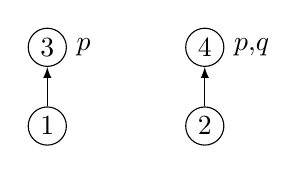
\begin{tikzpicture}[>=latex]
  \node (n1) at (0,0) [shape=circle,draw,inner sep=2pt, label=right:$$] {$1$} ;
  \node (n2) at (2,0) [shape=circle,draw,inner sep=2pt, label=right:$$] {$2$} ;
  \node (n4) at (0,1) [shape=circle,draw,inner sep=2pt, label=right:$p$] {$3$} ;
  \node (n5) at (2,1) [shape=circle,draw,inner sep=2pt, label=right:$p{,}q$] {$4$} ;
  \draw [->] (n1) -- (n4);
  \draw [->] (n2) -- (n5);
\end{tikzpicture}
\end{center}
%
donde $\rg\ l=\cset{p,q}$ y la valuaci\'on es definida como
$l(3)=\cset{p}, l(4)=\cset{p,q}, l(1)=l(2)=\cset{}$. Los valores iniciales de $S$ y $F$ son los que se muestran en
Tabla~\ref{tab:example}.

\begin{table}[ht]
\centering
{\footnotesize
\begin{tabular}{|c|c|c|c|c|}
\hline
&\multicolumn{2}{|c|}{Initial}&\multicolumn{2}{|c|}{Final}\\
$v$ & $S(v)$ & $F(v)$ & $S(v)$&$F(v)$\\
\hline
$1$ & $\{1,2,3,4\}$ & $\top$ & $\{1,2\}$&$\top\wedge\diam p$\\
$2$ & $\{1,2,3,4\}$ & $\top$ & $\{2\}$&$\top\wedge\diam(p\wedge q)$\\
$3$ & $\{3,4\}$ & $p$ & $\{3,4\}$ &$p$\\
$4$ & $\{4\}$ & $p\wedge q$ & $\{4\}$&$p\wedge q$\\
\hline
\end{tabular}
\caption{Valores iniciales y finales de $F$ y $S$}\label{tab:example}
}
\end{table}

Supongamos la siguiente ejecuci\'on:
\begin{enumerate}
\item Elegir $u=2,v=4,w=1$: detect that $1$ no simula $2$; set $S(2)=\{2,3,4\}$ y $F(2)=\top\wedge\diam(p\wedge q)$
\item Elegir $u=2,v=4,w=3$: detecta que $3$ no simula $2$; set $S(2)=\{2,4\}$ y $F(2)=\top\wedge\diam(p\wedge q)$
\item Elegir $u=2,v=4,w=4$: detecta que $4$ no simula $2$; set $S(2)=\{2\}$ y $F(2)=\top\wedge\diam(p\wedge q)$
\item Elegir $u=1,v=3,w=3$: detecta que $3$ no simula $1$; set $S(1)=\{1,2,4\}$ y $F(1)=\top\wedge\diam p$
\item Elegir $u=1,v=3,w=4$: detecta que $4$ no simula $1$; set $S(1)=\{1,2\}$ y $F(1)=\top\wedge\diam p$
\end{enumerate}
%After the fifth iteration it terminates. The final output is shown
%in Table~\ref{tab:example}. From this output one may conclude that,
%since $\simset_\subseteq(4)=\{4\}$, node $4$ has an \posre, namely
%$p\wedge q$. Node $2$ also has the \EL-RE $\top\wedge\diam(p\wedge
%q)$. In contrast $3$ does not have an \EL-RE because every
%$\pos$-formula true at $3$ is also true at $4$ (in this case, the
%only such possible formula is $p$ itself, or logically equivalent
%formulas such as $\top\wedge p\wedge p$). Nor $3$ has an \posre.

Despu\'es de la quinta iteraci\'on termina. Se muestra el resultado final
En la Tabla~\ref{tab:example}. A partir de esta salida se puede concluir que,
ya que$\simset_\subseteq(4)=\{4\}$, el nodo $4$ tiene un \posre, a saber,
$p\wedge q$. Nodo $2$ tambi\'en tiene la \EL-RE $\top\wedge\diam(p\wedge
q)$. En contraste $3$ no tiene un \EL-RE, porque cada
$\pos$-f\'ormula verdadera en $3$ tambi\'en es cierta en $4$ (en este caso, el
S\'olo tales f\'ormula posible es $p$ en s\'i mismos o equivalentes
f\'ormulas como $\top\wedge p\wedge p$). Tampoco $3$ tiene un \posre.

\end{ex}
\fi

\iffullversion
\newtheorem{teorema}{Teorema}
\begin{theorem}\label{thm:correctness-schematic-GRE}
Sea $S$ y $F$ la salida del Algoritmo
\ref{alg:schematic-GRE} con input $\gG=\tup{N,\to,l}$. Entonces para cada
nodo $v\in N$, $\interp{F(v)} = S(v) = \simset_\subseteq(v)$
\end{theorem}
\fi

\iffullversion
\begin{proof}
Es claro que para cada nodo $v\in N$,
$\simset_\subseteq(v)=S(v)$. Para la segunda parte, proponemos el siguiente invariante en el loop principal:
\begin{itemize}
\item[$I_1$:] para cada $v\in N$, $v \in \interp{F(v)}$
\item[$I_2$:] para cada $u,v\in N$, $\interp{F(u)} \subseteq S(u)$
\end{itemize}

Vamos a analizar el estado despu\'es de la inicializaci\'on, antes de la l\'inea~\ref{alg:line:loop-begin} se ejecuta por primera vez. En el uno
parte, es claro que para cualquier nodo $v\in N$, $v \in \interp{F(v)}$, as\'i
$I_1$ es verificado. Por otro lado, si $v\notin S(u)$ entonces
$l(u)\not\subseteq l(v)$ y hay un s\'imbolo proposicional $p$ tal que $p \in l(u)$ y $p \notin l(v)$. Desde que $v\notin\interp{p}$
entonces $v\notin\interp{\bigwedge l(u)}$ y as\'i
$v\notin \interp{F(u)}$.

Supongamos que $I_1$ y $I_2$ son verdaderos antes de ejecutar la 
l\'inea~\ref{alg:line:loop-body-begin}. Para todo $v\in N$ sea $S(v)=S_v$ y
$F(v)=\phi_v$ en este estado. Sean $u,v,w$ los nodos elegidos. Mostramos que el invariante es reestablesido luego de ejecutar la l\'inea
\ref{alg:line:loop-body-end-1}. Desde que $F$ y $S$ s\'olo cambian para $u$, 
es suficiente mostrar
\begin{itemize}
\item[$I_1'$:] $u \in \interp{\phi_u\wedge\diam \phi_v}$
\item[$I_2'$:] $\forall v\in N, \interp{\phi_u\wedge\diam \phi_v} \subseteq S_u\setminus\{w\}$
\end{itemize}
Para$I_1'$, es claro de $I_1$ que $u \in \interp{\phi_u}$ y $v \in \interp{\phi_v}$. Desde que $u\to v$ conclu\'imos que $u \in \interp{\diam
\phi_v}$.

Para $I_2'$ mostramos que para cualquier $v$, si $v\notin S_u\setminus\{w\}$
entonces $v\notin \interp{\phi_u\wedge\diam \phi_v}$. Si $v\notin S_u$,
por $I_2$ conocemos que $v\notin \interp{\phi_u}$ y entonces $v\notin
\interp{\phi_u\wedge\diam \phi_v}$. Supongamos que $v=w$ y, por
contradicci\'on, asumimos $v \in \interp{\phi_u\wedge\diam \phi_v}$.
Hay $w'\in N$ tal que $v\to w'$ y $w' \in
\interp{\phi_v}$. Por $I_2$ esto implica $w'\in S_v$. Aqu\'i $w'\in\su(w)\cap S_v$ y esto contradice la elecci\'on de $u,v,w$.

Cuando el algoritmo termina, $S=\simset_\subseteq$ y
el invariante $I_2$ implica que para cada $u,v\in N$,
$F(u) \subseteq \simset_\subseteq(u)$. Por otro lado, $I_1$
implica que $u \in \interp{F(u)}$ y por Proposici\'on \ref{prop:equiv} tenemos que si
 $v\in \simset_\subseteq(u)$ entonces $v \in \interp{F(u)}$.

Por lo tanto para cada $u,v\in N$, $\interp{F(u)} = \simset_\subseteq(u)$. 
As\'i que definiendo $\form:=F$ obtenemos el resultado deseado.
\end{proof}
\else
\fi

\iffullversion
\newtheorem{teorema}{Teorema}
\begin{theorem}
Algoritmo~\ref{alg:schematic-GRE} con input $\gG = \tup{N,\to,l}$
termina en tiempo
$O(\size{{\to}}^2\cdot\size{N}^3+\size{N}\cdot\size{\rg\ l})$.
\end{theorem}
\fi

\iffullversion
\begin{proof}
Para una implementaci\'on ingenua, el bucle principal se ejecuta en la mayor\'ia $\size{N}^2$ 
muchos pasos y para encontrar $u,v,w$ en
la l\'inea~\ref{alg:line:loop-begin} necesitamos $O(\size{N}\cdot\size{{\to}}^2)$

muchos pasos. El tiempo de ejecuci\'on del cuerpo del bucle es absorbida por este
\'ultima cantidad. Por lo tanto, en el tiempo total de ejecuci\'on del bucle principal es $O(\size{{\to}}^2\cdot\size{N}^3)$. Para cada $v\in N$, necesitamos
$O(\size{\rg\ l})$muchos pasos para las l\'ineas~\ref{alg:line:init1} y~\ref{alg:line:init2}. 
As\'i que en total, la inicializaci\'on toma $O(\size{N}\cdot\size{\rg\ l})$ 
muchos pasos.
\end{proof}
\else
\fi

\iffullversion
\begin{algorithm} \floatname{algorithm}{Algoritmo}\small
\io

\ForEach{$v\in \Delta$}{ $\prevS(v):=\Delta$

\If{para toda $r$ binaria, $\su{r}{v}=\emptyset$}{$S(v):=\{u\in \Delta
\mid \unary(v)\ \subseteq \unary(u) \}$

$F(v):=\bigwedge\unary(v)$ } \Else{ sea $r$ una relaci\'on binaria tal que $\su{r}{v}\not=\emptyset$

 $S(v):=\{u\in \Delta \colon
\unary(v) \subseteq \unary(u)\wedge\su{r}{u}\not=\emptyset \}$

$F(v):=\diam\top\wedge\bigwedge P(v)$ }}

\While{$\exists\ v\in \Delta:S(v)\not=\prevS(v)$}{

$\{\ I_1:\mbox{\bf assert\ }(\forall v)\ S(v)\subseteq\prevS(v)\ \}$

$\{\ I_2:\mbox{\bf assert\ }(\forall r,u,v,w)\
[(u,v)\in\interp{r}\wedge w\in
S(u)]\Rightarrow[\su{r}{w}\cap\prevS(v)\not=\emptyset]\ \}$

\ForEach{\mbox{\rm relaci\'on binaria $r$ y $u\in \pr{r}{v}$}}{

$remove := \pr{r}{\prevS(v)}\setminus\pr{r}{S(v)}$

$S(u):=S(u)\setminus remove$

\If{$\diam F(v)$ no es conjunci\'on de $F(u)$}{ $F(u):=F(u)\wedge
\diam F(v)$\label{alg:line:loop-body-end-2} } }

$\prevS(v)=S(v)$

} \caption{\small refinado $\EL$-similaridad y
\posre}\label{alg:refined-GRE}
\end{algorithm}
\fi

%Algoritmo \ref{alg:schematic-GRE} se puede modificar f\'acilmente para
%calcular la \ELAN-RE de cada conjunto de simulaci\'on $\simset_{\ELAN}$ 
%ajustando la inicializaci\'on: reemplazando $\subseteq$ por $=$ en la
%inicializaci\'on de $S(v)$ e inicializando $F(v)$ como
%$\bigwedge\left(\unary(v)\cup\overline \unary(v)\right)$,
%donde $\overline \unary(v)=\{\lnot p\mid v\notin\interp{p}\}$.


%Una implementaci\'on ingenua del Algoritmo~\ref{alg:schematic-GRE}

El Algoritmo~\ref{alg:schematic-GRE} puede ejecutar en un subconjunto arbitrario del dominio de $\tup{\Delta,\interp{\cdot}}$
 en $O(\size{\Delta}\times\size{\interp{\cdot}})$ pasos como se muestra en~\cite{HHK95}. Por lo tanto el problema \EL-GER se puede resolver en tiempo polinomial. N\'otese, sin embargo, que este resultado supone una representaci\'on conveniente de
f\'ormulas como, por ejemplo, grafos ac\'iclicos dirigidos, para asegurar que
cada paso de la construcci\'on de la f\'ormula puede hacerse en $O(1)$. %En
%\sect{size} vamos a echar un vistazo m\'as de cerca el tema y su relaci\'on con
%el tama\~no de los m\'as peque\~nos $\+L$-RE.

%Theorem~\ref{thm:complexity-EL-GRE} shows that there are efficient
%GRE algorihtms for \EL and \ELAN; languages which are --as discussed
%in \sect{choosinglanguage}-- generally simple to realize. The
%methods presented here, together with previous results
%of~\cite{AKS08} indicate that algorithms for computing
%$\+L$-simulator sets can, in many cases, be adapted to solve the
%$\+L$-GRE problem at no extra complexity cost.

%
%Algorithm~\ref{alg:schematic-GRE} was obtained by adding formula annotations
%to a standard `\EL-simulation-minimization' algorithm. Given an
%$\+L$-simulation-minimization, we can typically adapt it in an analogous
%way to obtain an $\+L$-GRE algorithm.
%The obtained algorithm computes $\+L$-REs for \emph{every} element of the
%domain simultaneously.
%This will make it particularly suitable for applications with
%static domains requiring references to many objects.


El Algoritmo~\ref{alg:schematic-GRE} se obtuvo mediante la adici\'on de anotaciones de f\'ormulas
al algoritmo est\'andar de `minimizaci\'on de \EL-simulaciones' presentado en la Secci\'on \ref{sec:indistinguiblesEL}. Dada una minimizaci\'on de
$\+L$-Simulaci\'on, podemos adaptarlo de
manera similar para obtener un algoritmo $\+L$-GER.
El algoritmo calcula las $\+L$-ERs para \emph{todos} los elementos del
dominio simult\'aneamente.
Esto har\'a que sea especialmente adecuado para aplicaciones con
dominios que requieren referencias a muchos objetos.

% but given its low complexity
%and the fact that termination is ensured (no risk of infinite regression, see~\cite{dale91:_gener_refer_expres_invol_relat}),
%it seems suitable for most applications.
 %Moreover, the algorithm can be adapted
%to dynamic domains by using techniques used to recompute simulations (see~\cite{saha:incre07}),
%so that only those RE that were affected by a change in the domain need to be
%recomputed.

%Por otra parte, el algoritmo se puede adaptar
%a dominios din\'amicos mediante el uso de t\'ecnicas que se utilizan para volver a calcular las simulaciones (vea~\cite{saha:incre07}),
%de modo que s\'olo las ERs que se vean afectadas por el cambio en el dominio necesitan ser recalculadas.
%
%We have not addressed so far other relevant issues of the
%GRE problem besides computational complexity. In particular,
%Algorithm~\ref{alg:schematic-GRE} pays no attention to the use of
%preferences among relations when generating an RE (i.e., preferring
%the selection of certain attributes over others, when possible).
%While there is room for improvement (e.g., making a weighted choice
%instead of the non-deterministic choice when choosing elements
%in the main loop of the algorithm), support for preferences is not
%one of the strong points of this family of algorithms.
%We consider algorithms with strong support for preferences in the following section.

%No hemos abordado hasta el momento otras cuestiones relevantes de la
%problema GER adem\'as de la complejidad computacional. En particular,
%Algoritmo~\ref{alg:schematic-GRE} no presta atenci\'on a la utilizaci\'on de
%preferencias entre las relaciones cuando se genera una ER (es decir, prefiriendo
%la selecci\'on de ciertos atributos por encima de otros, cuando sea posible).
%Si bien no hay margen de mejora (por ejemplo, hacer una elecci\'on ponderada
%en lugar de la elecci\'on no determinista a la hora de elegir los elementos
%en el bucle principal del algoritmo), el apoyo a las preferencias no es
%uno de los puntos fuertes de esta familia de algoritmos.
%Consideramos algoritmos con un fuerte apoyo a las preferencias en la siguiente secci\'on.


\section{Computando expresiones referenciales en $\alc$}
\label{sec:bisimulacion}

%Este algoritmo fue propuesto por %\cite{}
%
%La idea es transformar el problema de GER al problema de computar una f\'ormula de l\'ogica para la descripci\'on (DL) cuyos elementos que satisfagan la f\'ormula sea el conjunto target.% (o los elementos targets, en el caso de querer dar una ER para plurales aprovechando que una f\'ormula describe un conjunto que puede contener m\'as de un elemento).\\

A continuaci\'on daremos una introducci\'on a la l\'ogica para la descripci\'on \alc y la comparamos con \el. Las f\'ormulas $\varphi$ de $\alc$ son generadas por la siguiente gram\'atica:
$$
\varphi,\varphi' ::= \top \mid p \mid \neg \varphi \mid \varphi \sqcap \varphi'
\mid \exists R. \varphi
$$
donde $p$ es el conjunto de los s\'imbolos proposicionales \prop y $R$ es el de los s\'imbolos relacionales \rel. $\el$ puede definirse como $\alc$ sin negaci\'on. $\alc$ permite negaci\'on tanto at\'omica (e.g. $\neg \mathsf{flower}$) como sobre relaciones (e.g. $\neg \exists \mathsf{in}.\mathsf{hat}$).

Las f\'ormulas de $\alc$ (como las de $\el$) son interpretadas en modelos relacionales de primer orden $\gM = (\Delta,\interp{\cdot})$ donde
$\Delta$ es un conjunto no vac\'io y $\interp{\cdot}$ es una funci\'on de interpretaci\'on tal que:
$$
\begin{array}{ccl}
\interp{p} & \subseteq & \Delta  \mbox{ para $p \in \prop$}\\
\interp{R} & \subseteq & \Delta \times \Delta  \mbox{ para $R \in \rel$}\\
\interp{\neg \varphi} & = & \Delta - \interp{\varphi}\\
\interp{\varphi \sqcap \varphi'} & = & \interp{\varphi} \cap \interp{\varphi'}\\
\interp{\exists R.\varphi} & = & \{i \mid \mbox{para alg\'un } i', (i,i') \in \interp{R} \mbox{ e } i' \in \interp{\varphi} \}.\\
\end{array}
$$

\begin{figure}[t]
\begin{center}
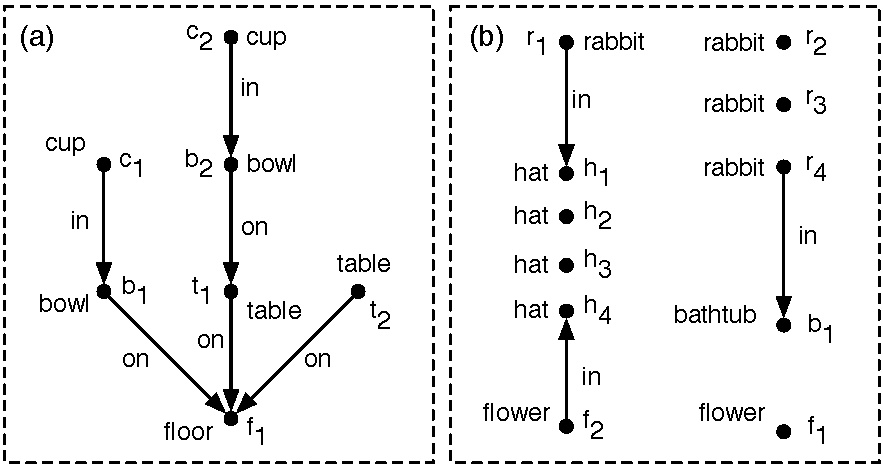
\includegraphics[width=8.5cm]{pic-dale-haddock.pdf}
\caption{}
\label{fig:dale-haddock}
\end{center}
\end{figure}


La interpretaci\'on de cada f\'ormula l\'ogica denota un conjunto de objetos del dominio; por lo tanto podemos usar f\'ormulas para describir conjuntos. 
Por ejemplo en el modelo de la Figura~\ref{fig:dale-haddock}(b), la f\'ormula
$\mathsf{flower}$ denota el conjunto $\{f_1,f_2\}$; La f\'ormula
$\mathsf{flower} \sqcap \exists \mathsf{in}.\mathsf{hat}$ denota
$\{f_2\}$; y la f\'ormula $\mathsf{flower} \sqcap \neg
\exists \mathsf{in}.\mathsf{hat}$ denota $\{f_1\}$.\\

En $\EL$ la similaridad no es una relaci\'on sim\'etrica. Por ejemplo, $f_1$ es \el-similar a $f_2$ en
Figura~\ref{fig:dale-haddock} (si $f_1$ satisface una f\'ormula, entonces tambi\'en la satisface $f_2$), pero $f_2$ no es \el-similar a $f_1$
($f_2$ satisface la f\'ormula $\exists \mathsf{in}.\mathsf{hat}$ y $f_1$
no la satisface). En \alc la similaridad es una relaci\'on sim\'etrica porque
el languaje contiene negaci\'on. En la figura, $f_1$ no es \alc-similar
a $f_2$ porque $f_2$ no satisface $\neg \exists
\mathsf{in}.\mathsf{hat}$. \alc\ es m\'as expresivo que \el,
esto es, para alg\'un elemento $a$ es posible ser \el-similar pero
no \alc-similar a alg\'un elemento $b$, pero no viceversa.

%%%
Como mostramos en la Secci\'on \ref{sec:seleccionandoLenguaje}, se puede demostrar que, para \ALC, los conjuntos de similaridad de un modelo finito
coinciden exactamente con las \emph{clases de simulaci\'on} del modelo. Las
clases de simulaci\'on se han estudiado ampliamente en la literatura
(por ejemplo,~\cite{BRV01}; \cite {Kurt:expr99}), y hay varios
algoritmos eficientes para el c\'alculo de las clases de \alc-simulaci\'on
\cite{hopc:algo71,paig:thre87,dovier04:_effic_algor_for_comput_bisim_equiv}.
Sin embargo, estos algoritmos s\'olo calculan las clases de simulaci\'on para \alc y no obtienen ERs como suced\'ia para \EL con los algoritmos que describimos en la Secci\'on \ref{sec:indistinguiblesEL}. Para poder generar ERs en \alc es necesario ampliar el algoritmo \cite{hopc:algo71} que
calcule junto con cada conjunto, tambi\'en una f\'ormula que denote
exactamente este conjunto.
 
El pseudoc\'odigo del algoritmo de \ALC que genera ERs se muestra como
Algoritmo~\ref{algo:bisim-3} (con $\gL=\alc$) y
Algoritmo~\ref{algo:bisim-add-alc}. Dado un modelo de $\gM=(\Delta,
\interp{\cdot})$, el algoritmo calcula un conjunto $\RE$ de $\alc$, las
f\'ormulas tales que $ \{\interp {\varphi} \mid \varphi \in \RE \} $ es el
conjunto de conjuntos \alc-similitud de $\gM$. El algoritmo comienza con $ \RE
= \{\top \} $ (donde $ \interp {\top} = \Delta $), y sucesivamente refina
$\RE$ haciendo que sus elementos denoten conjuntos m\'as y m\'as peque\~nos. Eso
mantiene el invariante que, al inicio y al final de cada iteraci\'on,
$\{\interp{\varphi} \mid \varphi \in \RE\}$ es siempre una partici\'on de
$ \Delta $. Los algoritmos iteran sobre todos los
s\'imbolos relacionales proposicionales en $ \prop $ y $\rel $ para la construcci\'on de nuevas f\'ormulas
hasta que todas las f\'ormulas de $RE$ denoten elementos \'unicos (es decir, que
s\'olo un individuo las satisfaga), o no se ha hecho ning\'un cambio desde la
 iteraci\'on anterior. En cada iteraci\'on, se llama al procedimiento
add$_\alc$ ($ \varphi $, $\RE$), que agrega $ \phi $ a toda
f\'ormula $\psi \in \RE $, 
si $\interp{\psi \sqcap \varphi} \not = \emptyset$ y $\interp{\psi \sqcap \neg \varphi} \not = \emptyset$.

El algoritmo \alc calcula los conjuntos \alc-similaridad del modelo en
tiempo $O(n^3)$, donde $ n $ es el n\'umero de individuos en el dominio. 
Por lo tanto su complejidad computacional es polinomial. En trabajo previo \cite{areces08} se ha mostrado que este algoritmo se ejecuta m\'as r\'apidamente que el algoritmo para \EL (ambos en tiempo polinomial).
El problema de \alc para la GER es que introducir\'a negaciones libremente en las distinciones de casos, esto
puede hacer que las f\'ormulas resultantes sean dif\'iciles de entender. 
Aqu\'i tambi\'en
presentamos un algoritmo para los conjuntos \el-similitud simplemente sustituyendo de la llamada a add$_{\alc} $ en
Algoritmo~\ref{algo:bisim-3} por una llamada a add$_{\EL} $, que es
definido en el Algoritmo~\ref{algo:bisim-add-el}. Como antes, el
algoritmo mantiene un conjunto $\RE = \{\varphi_1,\ldots,\varphi_n\}$ de
f\'ormulas (esta vez de \el) tal que $\interp{\varphi_1} \cup \ldots
\cup \interp{\varphi_n} = \Delta$, y que se refina de manera iterativa.
El algoritmo add$_{\alc}$ asegura que
$\interp{\varphi_1},\ldots,\interp{\varphi_n}$ es una partici\'on de
$ \Delta $, pero add$_{\EL}$ no lo asegura.

Debido a que mantiene un invariante m\'as d\'ebil, el conjunto \RE puede contener
m\'as f\'ormulas en el \el-algoritmo que en el \alc-algoritmo. Como $ \Delta $ tiene un n\'umero exponencial de subconjuntos,
hay un riesgo de que el \el-algoritmo podr\'ia tener peor tiempo de ejecuci\'on, como se muestra en trabajo previo \cite{areces08}.\\

 
\begin{algorithm}[H]\floatname{algorithm}{Algoritmo}
\dontprintsemicolon
\caption{Computando los conjuntos de $\mathcal{L}$-similaridad}
\label{algo:bisim-3}
\SetKwInOut{Input}{Entrada}\SetKwInOut{Output}{Salida}
\KwIn{Un modelo $\gM = (\Delta, \interp{\cdot})$}
\KwOut{Un conjunto \RE de f\'ormulas tales que
$\{\interp{\varphi} \mid \varphi \in \RE\}$ es el conjunto de
$\mathcal{L}$-similaridad de $\gM$.}

$\RE \leftarrow \{\top\}$

\For{$p \in \prop$}{
      add$_\mathcal{L}(p,\RE)$
   }

\While{exista alguna $\varphi \in \RE, |\interp{\varphi}|^\gM>1$}{
   \For{$\varphi \in \RE, R \in \rel$}{
         add$_\mathcal{L}(\exists R.\varphi,\RE)$
   }
   \If{no se hicieron cambios a \RE}{
      exit
      }
}
\end{algorithm}

\begin{algorithm}[H]\floatname{algorithm}{Algoritmo}
\caption{add$_\alc(\varphi,\RE)$}
\label{algo:bisim-add-alc}
\For{$\psi \in \RE$ with $|\interp{\psi}| > 1$}{
   \If{$\interp{\psi \sqcap \varphi} \not = \emptyset$ and
       $\interp{\psi \sqcap \neg \varphi} \not = \emptyset$}{
         add $\psi \sqcap \varphi$ and
               $\psi \sqcap \neg \varphi$ to \RE \;
         remove $\psi$ from \RE \;
      }
   }
\end{algorithm}

Vamos a probar estos algoritmos en algunos ejemplos. En primer lugar, corremos el \el algoritmo en el modelo que se muestra en la Figura~\ref{fig:dale-haddock} (a), que es
tomado de \cite{dale91:gener}. El
algoritmo comienza con $ \RE = \{\top \} $. En el primer bucle, se a\~naden
las f\'ormulas $\mathsf{floor}$, $\mathsf{bowl}$, $\mathsf{cup}$, y
$\mathsf{table}$, y luego se quita $\top$ porque est\'a subsumido.
No todas estas f\'ormulas denotan elementos \'unicos; por ejemplo,
$\interp{\mathsf{cup}}$ contiene dos elementos. As\'i que iteramos
las relaciones para refinar nuestras f\'ormulas. Despu\'es de la primera iteraci\'on sobre
las relaciones, tenemos  $\RE = \{ \mathsf{floor}, \mathsf{bowl} \sqcap
\exists \mathsf{on}.\mathsf{floor}, \mathsf{bowl} \sqcap \exists
\mathsf{on}.\mathsf{table}, \mathsf{cup}, \mathsf{table} \}$. Notar que
$\mathsf{bowl}$ fue subsumida por $\mathsf{bowl} \sqcap
\exists \mathsf{on}.\mathsf{floor}$ y $\mathsf{bowl} \sqcap \exists
\mathsf{on}.\mathsf{table}$, dos f\'ormulas que tienen interpretaciones singleton, es decir que son ERs de $b1$ y $b2$ respectivamente. Pero a\'un quedan sin distinguir $\mathsf{tables}$ y $\mathsf{cups}$.

%
\begin{algorithm}[t]\floatname{algorithm}{Algoritmo}
\dontprintsemicolon
\caption{add$_\el$($\varphi$, $\RE$)}
\label{algo:bisim-add-el}
\For{$\psi \in \RE$ with $|\interp{\psi}| > 1$}{
  \If{$\psi \sqcap \varphi$ is not subsumed in $\RE$ {\bf and}
    $\interp{\psi \sqcap \varphi} \neq \emptyset$ {\bf and}
    $\interp{\psi \sqcap \varphi} \neq \interp{\psi}$}{
    add $\psi \sqcap \varphi$ to $\RE$ \;
    borrar f\'ormulas subsumidas de $\RE$\;
  }
}
\end{algorithm}
Ahora podemos usar la divisi\'on entre los $\mathsf{bowls}$ para distinguir las $\mathsf{cups}$ en
la segunda iteraci\'on. El resultado de esto es $\RE = \{ \mathsf{floor},
\mathsf{bowl} \sqcap \exists \mathsf{on}.\mathsf{floor}, \mathsf{bowl}
\sqcap \exists \mathsf{on}.\mathsf{table}, \mathsf{cup} \sqcap \exists
\mathsf{in}. (\mathsf{bowl} \sqcap \exists
\mathsf{on}.\mathsf{floor}), \mathsf{cup} \sqcap \exists
\mathsf{in}. (\mathsf{bowl} \sqcap \exists
\mathsf{on}.\mathsf{table}), \mathsf{table} \}$. En este punto, todas las
f\'ormulas excepto $ \mathsf{table} $ denotan elementos \'unicos, y m\'as
iteraciones no nos permiten refinar $ \mathsf {table} $; por lo que el algoritmo
termina. Cada f\'ormula con una extensi\'on singleton es una expresi\'on referencial; por ejemplo, $\mathsf{cup} \sqcap \exists
\mathsf{in}. (\mathsf{bowl} \sqcap \exists \mathsf{on}.\mathsf{table})$ s\'olo es satisfecha por $ c_2 $, por lo que puede
realizarse como \textit{la taza que est\'a en el bowl, sobre la mesa}. Notar que
el algoritmo no se centr\'o en un elemento en particular (un target); sino que 
simult\'aneamente gener\'o ERs para todos los elementos a excepci\'on de las dos
mesas (que son \EL-similares entre s\'i).


El \el-algoritmo demora m\'as que el de \alc\ con el ejemplo de la Figura~\ref{fig:dale-haddock}(b) vea \cite{Stone1998a}. A pesar de ello
identifica correctamente a $r_1$ como \textit{el conejo en el sombrero} y a $ f_2$ como
\textit{la flor en el sombrero}. No es capaz de calcular una ER de $f_1$
porque $f_1$ es \el-similar a $f_2$. De hecho, el algoritmo
termina con $ \RE $ que contiene tanto a $\mathsf{flower}$ como a
$\mathsf{flower} \sqcap \exists \mathsf{in}.\mathsf{hat}$. Esto es un
patr\'on t\'ipico de los casos asim\'etricos de similitud en \EL: Si hay
dos f\'ormulas $ \varphi_1 $ y $ \varphi_2$ en el conjunto de salida con
$\interp{\varphi_1} \subset \interp{\varphi_2}$, entonces hay
en general, un elemento $b \in \interp{\varphi_2} -
\interp{\varphi_1}$ tal que todos los elementos en $\interp{\varphi_1} $ 
son similares a $ b $, pero no viceversa. Por el contrario, en el \alc-algoritmo puede explotar la mayor expresividad de \alc\ para dividir
$\mathsf{flower}$ en 2 nuevas f\'ormulas $\mathsf{flower} \sqcap
\exists \mathsf{in}.\mathsf{hat}$ y $\mathsf{flower} \sqcap \neg
\exists \mathsf{in}.\mathsf{hat}$, generando una ER \'unica para $f_1  $ pero que contiene negaci\'on.

\section{Computando expresiones referenciales en \FOL}
\label{sec:computandoEnFOL}
En esta secci\'on comenzaremos explicando trabajo previo en la GER usando $\FOL$. En particular describimos el trabajo de~\cite{graph} que se introdujo brevemente en la Secci\'on \ref{graph}. Luego mostraremos c\'omo la GER en $\FOL$ puede verse bajo la luz de las $\FOL$-simulaciones.
En~\cite{graph} introducen un algoritmo para GER basado en computaci\'on de \emph{isomorfismos de subgrafos}. Su algoritmo toma como entrada
un grafo dirigido etiquetado $G$ y un nodo $e$ (el target) y devuelve, si es posible,
un subgrafo conectado $H$  de $G$, que contiene $e$ y suficiente informaci\'on conectada para
distinguir a $e$ de los otros nodos.

Para mantener la terminolog\'ia de~\cite{graph}, en lo que sigue
podemos hablar alternativamente de \textbf{grafos etiquetados} en lugar de modelos relacionales, estos son esencialmente el mismo objeto matem\'atico. La diferencia es que los grafos etiquetados de \cite{graph} codifican las propiedades proposicionales utilizando
loops de relaciones binarias (por ejemplo, escriben $\nDog(e,e)$ en vez de $\nDog(e)$).

La idea principal de la implementaci\'on de~\cite{graph} de isomorfismos de subgrafos puede resumirse intuitivamente como sigue.
Dados dos grafos etiquetados $H$ y $G$, y los v\'ertices  $v$ de $H$
y $w$ de $G$, decimos que el par $(v, H)$ {\em refiere}
al par $(w, G)$ si y s\'olo si $H$ est\'a conectado y $H$ puede ser colocado ``sobre'' $G$ de tal manera que: 1) $v$ se coloca sobre $w$; 2) cada
nodo de $H$ se coloca sobre un nodo de $G$ con al menos los mismos
predicados unarios (pero tal vez m\'as); y 3) cada arista de $H$ es
colocada sobre una arista con la misma etiqueta. Por otra parte, $(v, H)$ {\em
refiere \'unicamente a} $(w, G)$ si $(v, H)$ refiere a $(w, G)$ y no hay
v\'ertice $w'\not=w$ in $G$ tal que $(v, H)$ refiere a $(w', G)$.

\begin{figure}[H]
\centering
\begin{tabular}{c@{\hspace{1.0cm}}c@{\hspace{1.0cm}}c@{\hspace{1.0cm}}}
\begin{picture}(45,50)
\put(0,0){\begin{tikzpicture}
  [
    n/.style={circle,fill,draw,inner sep=1.7pt,node distance=1.7cm},
    aSniffing/.style={->, >=stealth, semithick, shorten <= 3pt, shorten >= 3pt},
  ]
 \node[n,label=above:$v$,label=below:{\relsize{-1}$\begin{array}{c}\nFlower\\\ \end{array}$}] (a) {};
 \end{tikzpicture}}
 \end{picture}
&
\begin{picture}(35,50)
\put(0,0){\begin{tikzpicture}
  [
    n/.style={circle,fill,draw,inner sep=1.7pt,node distance=1.7cm},
    aIn/.style={->, >=stealth, semithick, shorten <= 3pt, shorten >= 3pt},
  ]
 \node[n,label=above:$v$,label=below:{\relsize{-1}$\begin{array}{c}\nHat\\\ \end{array}$}] (a) {};
 \end{tikzpicture}}
 \end{picture}
&
\begin{picture}(70,50) \put(0,0){\begin{tikzpicture}
  [
    n/.style={circle,fill,draw,inner sep=1.5pt,node distance=1.5cm},
    aIn/.style={->, >=stealth, semithick, shorten <= 3pt, shorten >= 3pt},
  ]
 \node[n,label=above:,label=below:{\relsize{-1}$\begin{array}{c}\nHat\\\ \end{array}$}] (a) {};

 \node[n,label=above:$v$,label=below:{\relsize{-1}$\begin{array}{c}\nFlower\\\ \end{array}$}, right of=a] (b) {};

 \draw [aIn,bend right=40] (b) to node[auto,swap]{\relsize{-1}$\aIn$} (a);

 \end{tikzpicture}}
 \end{picture}
\vspace{-.2cm}\ \\
(i)&(ii)&(iii)
\end{tabular}
 \caption{Algunos subgrafos conectados de la escena de la Figura~\ref{fig:dale-haddock}, \label{fig:subgraphs} (i) puede realizarse como  \emph{flor},  (ii) como \emph{sombrero} y (iii) \emph{flor en un sombrero}. }
 \end{figure}

Como ejemplo, consideremos el modelo relacional que se representa en la
Figura~\ref{fig:dale-haddock} como un grafo etiquetado $G$, y consideremos los pares de nodos conectados y subgrafos $(V, H)$ que se muestran en 
la Figura~\ref{fig:subgraphs}. Est\'a claro que (i) se refiere a cualquier nodo $w\in\{f_1,f_2\}$; (ii) se refiere a $w\in\{h_1,h_2,h_3,h_4\}$
y en (iii) el hat refiere \'unicamente a $h_4$, y flower a $f_2$; 
El algoritmo propuesto en~\cite{graph} es una
implementaci\'on directa del algoritmo de {\bf \emph{branch \& bound}} guiado por costo que trata sistem\'aticamente todos los
subgrafos pertinentes $H$ de $G$ comenzando con el subgrafo
que contiene s\'olo el v\'ertice target $v$ y ampliando de forma recursiva, tratando de
agregar arcos de $G$ que son adyacentes al subgrafo $H$ constru\'ido
hasta el momento. En la terminolog\'ia de~\cite{graph} un {\em distractor} es un nodo de $G$ diferente de
$v$ que tambi\'en es referenciado por $H$.
El algoritmo asegura que un subgrafo se refiere \'unicamente al target $v$ cuando no hay distractores. Llegado este punto, existe una
soluci\'on, pero puede haber otra
soluci\'on de menor costo por lo que el proceso de b\'usqueda contin\'ua hasta que
se detecta la soluci\'on de menor costo. 
La relaci\'on entre el m\'etodo basado en grafos
de~\cite{graph} y nuestra perspectiva de teor\'ia de modelos: en
modelos relacionales finitos, el isomorfismo de subgrafos corresponde a las
\EPFOL-simulaciones. Dados nodos $u,v$ de
$G$, existe un subgrafo isomorfo a G a trav\'es de $f$, que contiene $ u $ y
$v$, y tal que $f(u)=v$ si y s\'olo si $u \simul{\+\EPFOL} v$. Una implementaci\'on usando $\+\EPFOL$-simulaciones se muestra en el Algoritmo \ref{alg:makeRE}.
%
%Despu\'es de haber explicitado esta noci\'on de igualdad y, con ella, la de
%lenguaje l\'ogico asociado a ella, podemos proceder a generalizar el
%algoritmo para hacer que funcione para otros lenguajes, y adaptarlo para
%ordenar a la salida de una f\'ormula en lugar de un grafo. Esto se muestra en los
%Algoritmos~\ref{alg:makeRE} y~\ref{alg:find}.
%
%\begin{center}\begin{minipage}[t]{5.1cm}%
%algoritmo 3

\begin{algorithm}%[H]
\floatname{algorithm}{Algoritmo}\small
\SetKwFunction{makeRE}{makeRE$_\FOL-$}
\SetKwFunction{findGraph}{find$_\FOL-$}
\SetKwFunction{init}{init_$\FOL-$}
\SetKwFunction{buildF}{buildF$_\FOL-$}

%$v_H$ := \emph{new node}\;

\SetKwInOut{Input}{Entrada}\SetKwInOut{Output}{Salida}
\Input{$G=\tup{\Delta_G,\interp{\cdot}}$ y $v\in\Delta_G$}
\Output{$\+\EPFOL$-ER para $v$ en $G$ si hay, o $\bot$}
\BlankLine

\vspace{3.0pt}

\BlankLine

$H$ := $\tup{\cset{v},\emptyset}$\; $f$ := $\cset{v \mapsto v}$\;
$H'$ := \findGraph($v, \bot, H, f$)\;
\BlankLine

%\texttt{buildF}$_\EPFOL(H',v)$}\label{alg:build-form-epfol}
%\textbf{let}
$H' = \tup{\cset{a_1\ldots a_n}, \interp{\cdot}}$,$v=a_1$\;
\tcp{let $v=a_1$}
$\gamma$ := $\displaystyle \bigwedge_{\mathclap{a_i \neq a_j}} (x_i
\not\approx x_j) \land \bigwedge_{\mathclap{(a_i,a_j) \in
\interp{r}}} r(x_i,x_j) \land \bigwedge_{\mathclap{a_i \in
\interp{p}}}p(x_i)$

\BlankLine
\vspace{2.2pt}
\Return{$\exists x_2\ldots \exists x_n . \gamma$}\;

%\Return{\buildF$(H',v)$}\;
\caption{\small \texttt{makeRE}$_\FOL-$($v$)}\label{alg:makeRE}
\end{algorithm}


%fin algoritmo 3
\hspace{.05cm}
 % \begin{minipage}[t]{6.8cm}%

%empieza algoritmo 4
\begin{algorithm}[H] 
\floatname{algorithm}{Algoritmo}\small
\SetKwFunction{findGraph}{find$_\+L$} 
\SetKwFunction{cost}{cost}
\SetKwFunction{matchGraph}{match$_\+L$}
\SetKwFunction{extendGraph}{extend$_\+L$}

\If{$\mathit{best} \neq \bot \land \cost(\mathit{best}) \leq
  \cost(H)$}{
  \Return $\mathit{best}$\;} 
$\mathit{distractors}$ := $\cset{n \mid n \in \Delta_G, n \neq v , v \simul{\+L} n}$\;

\If{$\mathit{distractors} = \emptyset$}{\Return $H$\;}

 $A$ := $\cset{H {+} p(u) \mid u \in \Delta_H, u \in \interp{p}_G  \setminus \interp{p}_H}$\;

 $B$ := $\cset{H {+} r(u,v) \mid u \in \Delta_H, \{(u,v),(v,u)\}\cap \interp{r}_G \setminus \interp{r}_H\not=\emptyset}$\;

 $EXT$ :=$(A \cup B) \times \cset{\mathit{id}}$\;
%
%
\ForEach{$\tup{H',f'} \in EXT$}{
  $I$ := \findGraph($v,\mathit{best},H', f'$)\;
  \If{$\mathit{best} = \bot \lor \cost(I) \leq \cost(\mathit{best})$}{$\mathit{best} := I$}
}
 
\Return{$\mathit{best}$}\;

\caption{\small \texttt{find}$_\FOL-$($v, \mathit{best},H,f$)}\label{alg:find}
\end{algorithm}
  %\end{minipage}%
%\end{center}


El primero transforma el {\em grafo} calculado, que se refiere \'unicamente al target $v$ en una $\+L$-ER {\em
f\'ormula para} $v$; \'este \'ultimo nos dice c\'omo extender $H$ en cada paso
del bucle principal del Algoritmo~\ref{alg:find}. Hay que tener en cuenta que, a diferencia de la
presentaci\'on de~\cite{graph}, \instFun{makeRE}{\FOL} computa
no s\'olo un grafo $H$, sino tambi\'en una $\+L$-Simulaci\'on de $f$.

Como nota final sobre la complejidad, la computaci\'on
\EPFOL-distractores parece requerir necesariamente una soluci\'on al problema de isomorfismos de subgrafos, que es NP-completo). Mientras que en la Secci\'on \ref{sec:greViaSimulacion} y \ref{sec:bisimulacion} presentamos algoritmos que pueden encontrar ERs en tiempo polinomial.
%en ~ \ secta {tama\~no}.


%%ROMI---
\section{Notas finales y linkeo del cap\'itulo}
\label{sec:notasFinales}

En este cap\'itulo dimos definiciones b\'asicas de modelo, interpretaci\'on, f\'ormula y de otros conceptos b\'asicos de l\'ogica y teor\'ia de modelos. Explicamos e ilustramos la noci\'on de similaridad de 2 elementos $u$ y $v$ de un lenguaje l\'ogico $\+L$ ($u \simil{\+L} v$ en el lenguaje $\+L$). Cuando para toda f\'ormula $\phi \in \+L$, tenemos que $\{u,v\} \subseteq \interp{\phi}$,  se dice que $u$ y $v$ son indistinguibles en el lenguaje l\'ogico $\+L$. Como la similaridad est\'a definida para infinitas f\'ormulas, tambi\'en vimos un teorema que cuando el modelo sea finito acota esa b\'usqueda
infinita a una finita, teniendo en cuenta propiedades de las l\'ogicas usadas. Explicamos algoritmos eficientes que computan ERs usando simulaciones en \FOL, \ALC y \EL. Tambi\'en se mostr\'o una clasificaci\'on de los algoritmos vistos seg\'un la complejidad computacional de los mismos. 

En el Cap\'itulo \ref{sec:algoritmo} extenderemos estos algoritmos integrando una distribuci\'on finita de probabilidades que representa la incertidumbre presente en posibles aplicaciones de la generaci\'on de expresiones referenciales que deben referirse al mundo real y tienen que lidiar con datos ruidosos de sensores y modelos incompletos de la realidad. El objetivo es generar un ranking de las expresiones referenciales ordenado por la probabilidad de ser correctamente interpretada en el contexto. En el Cap\'itulo \ref{sec:evaluacion} evaluamos estos algoritmos usando t\'ecnicas autom\'aticas y evaluaciones de jueces humanos sobre datos de benchmarks del \'area. En el Cap\'itulo \ref{sec:corpus} se realiza una evaluaci\'on con respecto a un nuevo corpus de expresiones referenciales de puntos de inter\'es en mapas de ciudades con distintos niveles de zoom. 



%En este cap\'itulo dimos definiciones b\'asicas de modelo, 
%interpretaci\'on, f\'ormula, hablamos de la noci\'on de similaridad de 2 elementos $u$ y $v$ del modelo la cual dice que son 
%similares en $\+L$ ($u \simil{\+L} v$ en el lenguaje $+L$), cuando para toda f\'ormula $\phi \in \+L$, tenemos que 
%$\{u,v\} \subseteq \interp{\phi}$, no hay una f\'ormula que satisfaga uno y no el otro, por lo tanto se dice que son indistinguibles en el lenguaje l\'ogico $\+L$. Como las similaridad est\'a definida para infinitas f\'ormulas, tambi\'en vimos un teorema que bajo ciertas condiciones (que el modelo sea finito) acota esa b\'usqueda infinita a una finita, teniendo en cuenta propiedades de las l\'ogicas usadas. Computamos ERs en \FOL, \ALC y \EL. Tambi\'en se mostr\'o una clasificaci\'on de los algoritmos vistos seg\'un la complejidad computacional de los mismos. Explicamos como computamos las ERs para los distintos lenguajes l\'ogicos \FOL, \ALC y \EL. Elegimos para nuestro algoritmo el lenguaje \EL ya que es el lenguaje que restringe la expresividad a la encontrada en corpora.%es decir que no existe otro elemento en el modelo el cual sea 
